\documentclass[oneside, article]{memoir}

% \usepackage{bibte?}
% \addbibresource{measurement-error-gp.bib}

\usepackage[utf8]{inputenc}
\usepackage{lmodern}

\usepackage{amsmath, amsthm, amsfonts, amssymb, mathtools, commath,
hyperref, cancel, bm}
\usepackage{doi, xcolor}
% \usepackage[T1]{fontenc}

% \usepackage{eulervm}
\usepackage[tracking, spacing]{microtype}
\usepackage[margin=1in]{geometry}
\usepackage{algorithm,algpseudocode, algorithmicx}
\microtypecontext{spacing=nonfrench}
\newtheorem{definition}{Definition}
\newtheorem{proposition}{Proposition}
\newtheorem{conjecture}{Conjecture}
\newtheorem{theorem}{Theorem}
\newtheorem{problem}{Problem}
\newtheorem{corollary}{Corollary}
\newtheorem{remark}{Remark}
\newtheorem{lemma}{Lemma}
\newtheorem{example}{Example}
\DeclareMathOperator{\trace}{\operatorname{tr}}
\DeclareMathOperator{\expect}{\mathbb{E}}
\DeclareMathOperator{\probability}{\mathbb{P}}
\DeclareMathOperator{\Var}{\operatorname{Var}}
\DeclareMathOperator{\Cov}{\operatorname{Cov}}
\begin{document}
% Analytic filtering for single-layer RBF dynamics:
% \cite{deisenroth_analytic_2009}

\chapter{Notation}
The vector \(e_i\) has a 1 in the \(i\)th place and zeros everywhere else.

When \(\sigma:\mathbb R \to \mathbb R\) is a neural network activation function, \(\sigma (x)\) for \(x \in \mathbb{R}^n\) is applied elementwise.

The variance-covariance matrix of a random vector \(X\) is \(\Var X = \expect(X - \expect X)(X - \expect X)^\intercal\).

We use a highly stylized notation to depict state dynamics.
Lowercase letters \(\{x_t\}\) refer to a realization of a stochastic process.
Statements with an equals sign such as \(x_{t} = F(x_{t-1}) +
\eta_t\) are ``strong,'' i.e.~hold almost surely.

Uppercase letters such as \(\{X_t\}\) refer to probability laws.
Statements with a \(\Longleftarrow\) such as \(X_t \Longleftarrow
F(X_{t-1})\) are ``weak'' and denote propagation of uncertainty (the
approximation of which is a key contribution of this paper): \(X_t\)
is the distribution of \(F(X_{t-1})\).
In expressions such as \(H(X_t) + \mathcal N(0, R)\), we mean that
the noise term is independent of all other randomness.

The comma \(,\) is a higher-order function:
if \(x \mapsto f(x)\) and \(x \mapsto g(x)\) are functions, then \((f
, g)\) is the function \(x \mapsto (f(x), g(x))\).

The direct sum of two square matrices \(A\) and \(B\) is denoted by
\(A \oplus B\) and refers to the block-diagonal matrix \(A \oplus B =
  \begin{pmatrix} A & 0 \\ 0 & B
\end{pmatrix}\).

In algorithmic pseudocode, a \emph{Function} is a pure function in
the mathematical or functional
programming sense.
In particular, the variable names are meaningless placeholders.
\(f(x) = x^2\) defines the same function as \(f(y) = y^2\).
A \emph{Procedure} is code that generates ``side effects.''
Inside a procedure, the variable names are meaningful and refer to
the same variables used to pose an algorithmic problem.

\chapter{Background: prediction, filtering, and smoothing of
nonlinear stochastic systems}
A dynamic system is described by
\begin{subequations}
  \label{eq:dynamic-system}
  \begin{align}
    x_0 &\sim \mathcal{N}(\mu_0, \Sigma_0) \\
    x_t &= F(x_{t-1}, u_t) + \eta_t, &\eta_t &\sim \mathcal{N}(0, Q)
    & \forall t &\in \cbr{1 \ldots T}\\
    y_t &= H(x_t, u_t) + \epsilon_t, &\epsilon_t &\sim \mathcal{N}(0,
    R) & \forall t &\in \cbr{1 \ldots T}
  \end{align}
\end{subequations}
where \(x_t \in \mathbb{R}^{n_x}\) is the state, \(u_t \in \mathbb
R^{n_u}\) is the input, and \(y_t \in \mathbb{R}^{n_y}\) is the output.
The random variables \(x_0\), \(\{\eta_t\}_{t=1}^T\), and
\(\{\epsilon_t\}_{t=1}^T\) are independent.

From this model three classic problems emerge.
\begin{problem}[Prediction]\label{problem:prediction}
  Given \(\{u_s\}_{s=0}^{t-1}\) and \(\{y_s\}_{s=1}^{t-1}\), predict
  \(x_t\) and \(y_t\) as a joint distribution \((\hat X_{t \mid t-1},
  \hat Y_{t \mid t-1})\).
\end{problem}

\begin{problem}[Filtering]\label{problem:filtering}
  Given \(\{u_s\}_{s=0}^{t}\) and \(\{y_s\}_{s=1}^t\), estimate
  \(\hat X_{t \mid t}\).
\end{problem}

\begin{problem}[Smoothing]\label{problem:smoothing}
  Given \(\{u_s\}_{s=0}^T\) and \(\{y_s\}_{s=1}^T\), estimate \(\hat X_{t \mid T}\).
\end{problem}
In the case that \(F\) and \(H\) are linear functions,
the Kalman filter Alg.~\ref{alg:kalman-filter} solves the prediction
and filtering problems by a forward recursion, and the
Rauch-Tung-Striebel smoother Alg.~\ref{alg:rts-smoother} solves the
smoothing problem by a backward recursion.
We have stylized these algorithms in order to highlight their
Bayesian motivation and to establish abstractions that put many
different types of nonlinear Kalman filters on the same footing.

\begin{algorithm}
  \caption{
    \label{alg:kalman-filter}
    General Kalman algorithm for recursive \textbf{prediction} (problem
    \ref{problem:prediction}) and \textbf{filtering} (problem
  \ref{problem:filtering})}
  \begin{algorithmic}[1]
    \Require State transition function \(F\) and observation model \(H\)
    \Require State covariance \(Q\) and and observation covariance \(R\)
    \Require Uncertainty propagation operator ``\(\Longleftarrow\)''
    \Function{Predict}{$X, u$}
    \State
    \(X' \Longleftarrow F(X, u) + \mathcal{N}(0, Q)\)
    \Comment{Propagate \(X\) through state transition}
    \State
    \(((X', u), Y') \Longleftarrow (\text{id}, H)(X', u) +
    \mathcal{N}(0, 0_{n_x} \oplus R)\)
    \Comment{Propagate \(X'\) through observation model}
    \State\Return \((X', Y')\)
    \Comment{Joint distribution of next state and next output}
    \EndFunction
    \Function{Update}{$(X, Y), y$}
    \State
    \((X', y) \Longleftarrow\) conditional distribution of \((X,Y)\)
    given \(Y=y\)
    \Comment{Apply Bayes' rule}
    \State\Return \(X'\)
    \EndFunction
    \Procedure{Filter}{$u_1, \ldots, u_t, y_1, \ldots, y_t$}
    \State \(\hat X_{0 \mid 0} \Longleftarrow \mathcal{N}(\mu_0, \Sigma_0)\)
    \For{$k \in \cbr{1 \ldots t}$}
    \State \( (\hat X_{k \mid k-1}, \hat Y_{k \mid k-1})
    \Longleftarrow \textsc{Predict}(\hat X_{k-1 \mid k-1}, u_k) \)
    \Comment{Solution to problem \ref{problem:prediction}}
    \State \( \hat X_{k \mid k}  \Longleftarrow \textsc{Update}((\hat
    X_{k \mid k-1}, \hat Y_{k \mid k-1}), y_k) \)
    \Comment{Solution to problem \ref{problem:filtering}}
    \EndFor
    \EndProcedure
  \end{algorithmic}
\end{algorithm}

\begin{algorithm}
  \caption{
    \label{alg:rts-smoother}
    General RTS algorithm for recursive \textbf{smoothing} (problem
  \ref{problem:smoothing})}
  \begin{algorithmic}[1]
    \Require State transition function \(F\)
    \Require State covariance \(Q\)
    \Require Uncertainty propagation operator ``\(\Longleftarrow\)''
    \Function{Predict}{$X, u$}
    \State
    \(((X, u), X') \Longleftarrow (\text{id} , F)(X, u) +
    \mathcal{N}(0, 0 \oplus Q)\)
    \Comment{Propagate \(X\) through state transition}
    \State\Return \((X, X')\)
    \Comment{Joint distribution of current state and next state}
    \EndFunction
    \Function{Update}{$(X, X'), X''$}
    \State
    \((X, X'') \Longleftarrow\) conditional distribution of
    \((X,X')\) given \(X' = X''\)
    \Comment{Apply Bayes' rule}
    \State\Return \(X\)
    \EndFunction
    \Procedure{Smooth}{$u_1, \ldots, u_T, y_1, \ldots, y_T$}
    \State \(\{\hat X_{k|k}\}_{k=1}^T \Longleftarrow
    \textsc{Filter}(u_1, \ldots, u_T, y_1, \ldots, y_T)\)
    \For{$k \in \cbr{T-1 \ldots 0}$}
    \State \( (\hat X_{k|k}, \hat X_{k+1|k}) \Longleftarrow
    \textsc{Predict}(\hat X_{k \mid k}, u_{k+1}) \)
    \State \( \hat X_{k|T} \Longleftarrow \textsc{Update}((\hat
    X_{k|k}, \hat X_{k+1|k}), \hat X_{k|T}) \)
    \Comment{Solution to problem \ref{problem:smoothing}}
    \EndFor
    \EndProcedure
  \end{algorithmic}
\end{algorithm}

In both filtering and smoothing, the operations of \textsc{Predict}
and \textsc{Update} are implemented as pure functions whose contract
(input and output) are probability distributions.
We enforce a functional distinction between \emph{how} uncertain
belief is generated (using the \(\Longleftarrow\) operator) and
\emph{what} operations (marginalizing or conditionalizing) are
carried out on the resulting belief.
% \footnote{
This segregation of responsibilities naturally translates to
idiomatic encapsulation in the object-oriented Python implementation.
For example, the \textsc{Predict} method reads:

\begin{minipage}{\textwidth}
\begin{verbatim}
def predict(self, x: Normal, method="analytic"):
      """Predicts the next state and output given the current state,
          using the uncertainty propagation given by `method`"""
      # predict state
      x_pred = self.F(x, method=method).add_covariance(self.Q)
      # predict joint distribution of state and output
      x_and_y_pred = self.H.augment_with_identity()(
          x_pred, method=method
      ).add_covariance(self.R, at=self.OUTPUTS)
      return x_and_y_pred
\end{verbatim}
\end{minipage}
If \eqref{eq:dynamic-system} is a linear system in state space \((A,
B, C, D)\) form,
uncertainty propagation is exact, and all of the random variables are
jointly Gaussian.
The \textsc{Predict} function of Alg.~\ref{alg:kalman-filter} would read:
\begin{algorithmic}
  \Function{Predict}{$X \sim \mathcal N\del{\hat x, P_{xx}}, u$}
  \State \(\hat x' \gets A \hat x + B u\)
  \State \(P_{xx}' \gets A P_{xx} A^\intercal + Q\)
  \State \(\hat y' \gets C \hat x + D u\)
  \State \(P_{yy}' \gets C P_{xx}' C^\intercal + R\)
  \State \(P_{xy}' \gets P_{xx}' C^\intercal\)
  % \State \Return \((\hat x', \hat y, P_{xx}', P_{yy}, P_{xy})\)
  \State \Return \(
    \begin{pmatrix} X' \\ Y'
    \end{pmatrix} \sim \mathcal N \del{
      \begin{pmatrix} \hat x' \\ \hat y'
      \end{pmatrix},
      \begin{pmatrix} P_{xx}' & P_{xy}' \\ P_{xy}'^\intercal & P_{yy}'
  \end{pmatrix}}\)
  \EndFunction
\end{algorithmic}

\section{Extension to nonlinear systems}
When \(F\) is a nonlinear function, the pushforward probability law
of \(F(X, u)\), where \(X \sim \mathcal{N}(\mu, \Sigma)\) and \(u\)
is deterministic, is not necessarily Gaussian.
This is a challenging problem for Bayesian inference, because the
\text{Update} functions of Alg.~\ref{alg:kalman-filter} and
Alg.~\ref{alg:rts-smoother} can be hard to implement without prior conjugacy.
Assumed Density Filtering approximates \(F(X)\) (hereafter the
arguments to \(F\) are lumped together as a single Gaussian variable)
with a Gaussian distribution:
\begin{align*}
  F(X)
  \approx \mathcal{N}\del{\expect F(X), \Var F(X)}
\end{align*}
This distributional approximation can be viewed as maximum entropy
(forgetting the higher-order moments of \(F(X)\)) or as variational
inference (minimizing the KL divergence between \(F(X)\) and the
Gaussian approximation).
But \(\expect F(X)\) and \(\Var F(X)\) have in general no closed form.
\begin{itemize}
  \item Particle Filtering evaluates these moments using Monte Carlo
    integration.
    With an unlimited computational budget, it is possible to get
    arbitrarily close to exactness.
  \item The Extended Kalman Filter and second-order Extended Kalman
    Filter evaluate these moments analytically by applying a Taylor
    expansion to \(F\).
    These methods fail for highly nonlinear \(F\) that are poorly
    approximated by local asympototics.
  \item The Unscented and Cubature Kalman Filters evaluate these
    moments numerically by approximating the continuous Normal
    distribution of \(X\) using \(O(n_x)\) point masses.
    % But these numerical integration schemes struggle with highly
    % nonlinear \(F\).
    This amounts to a striking order reduction in light of the fact
    that the number of points needed for accurate numerical
    quadrature of a function \(F(X)\) is in general exponential in \(n_x\).
    This simplification is justified in the case of the Unscented
    Transform\footnote{cite Uhlmann (1997)} using analytic regularity of \(F\).
    Thus it stands to reason that reduced-order discretizations of
    \(X\) struggle to integrate highly nonlinear \(F\).
\end{itemize}

{\color{red} review pros and cons here? computational complexity,
point accuracy, and coverage}

In our work, \(F\) and \(H\) are multi-layer neural networks.
At each layer, we re-impose the variational Gaussian approximation,
which allows us to calculate the mean and variance of the output
analytically, as described in the next section.

\chapter{Uncertainty propagation through neural networks}
Suppose that a function \(f\) is represented by a neural network with
\(\ell\) layers:
\begin{subequations}
  \label{eq:neural-network}
  \begin{align}
    f(x) &= f^\ell(x), \\
    f^k(x) &= g(f^{k-1}(x); A^k, b^k, C^k, d^k), & k \in \cbr{1 \ldots \ell},
    \label{eq:hidden-layer}
    \\
    f^0(x) &= x
  \end{align}
\end{subequations}
Here, \(\{(A^k, b^k, C^k, d^k)\}_{k=1}^\ell\) are parameters,
\(\sigma\) is a nonlinear activation function, and the layer function is
\begin{align}
  g(x; A, b, C, d) = \sigma(A x+ b) + C x + d.
\end{align}

The uncertainty propagation problem is:
\begin{problem}
  Let \(f\) be given by \eqref{eq:neural-network}.
  Given \(X \sim \mathcal N(\mu, \Sigma)\), find the Normal random
  variable \(Y\) such that
  \begin{align*}
    Y \sim \mathcal N\del{\expect f(X), \Var f(X)}.
  \end{align*}
\end{problem}

Our approach is to approximate each hidden layer
\eqref{eq:hidden-layer} by a Gaussian distribution:
\begin{subequations}
  \label{eq:neural-network-gaussian}
  \begin{align}
    Y &\Longleftarrow Y^\ell
    \\
    Y^k &\Longleftarrow g(Y^{k-1}; A^k, b^k, C^k, d^k), & k \in
    \cbr{1 \ldots \ell},
    \label{eq:hidden-layer-gaussian}
    \\
    Y^0 &\Longleftarrow X
  \end{align}
\end{subequations}
Now we have reduced the problem to that of Gaussian propagation
through one hidden layer at a time.
We have to find the mapping
\begin{align}
  % Y &\Longleftarrow g(X; A, b, C, d),
  % \intertext{by which we mean}
  Y &\approx \mathcal{N}\del{\expect g(X; A, b, C, d), \Var g(X; A, b, C, d)}
\end{align}
in distribution.

\begin{definition}
  \label{def:moment-maps}
  Given a nonlinear function \(\sigma: \mathbb{R} \to \mathbb R\),
  the functions \(M_\sigma: \mathbb{R}  \times \mathbb{R}_+ \to
  \mathbb{R}\) and \(K_\sigma, L_\sigma: \mathbb{R}^2 \times \mathbb
  R_+^2 \times [0, 1] \to \mathbb{R}\) are
  \begin{align*}
    M_\sigma(\mu; \nu) &= \expect{\sigma(X)},
    & X &\sim \mathcal N(\mu, \nu)
    \\
    K_\sigma(\mu_1, \mu_2; \nu_{11}, \nu_{22}, \nu_{12}) &= \Cov
    (\sigma(X_1), \sigma(X_2)),
    &
    \begin{pmatrix}
      X_1 \\ X_2
    \end{pmatrix} &\sim \mathcal N\del{
      \begin{pmatrix}
        \mu_1 \\ \mu_2
      \end{pmatrix},
      \begin{pmatrix}
        \nu_{11} & \nu_{12} \\
        \nu_{12} & \nu_{22}
      \end{pmatrix}
    }
    \\
    L_\sigma(\mu_1; \nu_{11}, \nu_{22}, \nu_{12}) &= \Cov
    (\sigma(X_1), X_2),
    &
    \begin{pmatrix}
      X_1 \\ X_2
    \end{pmatrix} &\sim \mathcal N\del{
      \begin{pmatrix}
        \mu_1 \\ \star
      \end{pmatrix},
      \begin{pmatrix}
        \nu_{11} & \nu_{12} \\
        \nu_{12} & \nu_{22}
      \end{pmatrix}
    }
    \\
  \end{align*}
\end{definition}

When \(\sigma\) is differentiable, \(L_\sigma\) can be computed using:
\begin{lemma}[Stein's lemma]
  \label{lem:stein}
  Let \(L_\sigma\) be defined as in Definition \ref{def:moment-maps}.
  Then
  \begin{align*}
    L_\sigma(\mu_1, \mu_2; \nu_1^2, \nu_2^2, \rho) &= \rho
    \nu_1 \nu_2 \expect \sigma'(Z_1),
    & Z_1 &\sim \mathcal N(\mu_1, \nu^2_1).
  \end{align*}
\end{lemma}

% A consequence of Stein's Lemma is

We can use the trio of functions \(M_\sigma, K_\sigma, L_\sigma\) to
compute the moments of \(g(X; A, b, C, d)\):
\begin{lemma}
  Let \(g\) be the function defined by \(g(x; A, b, C, d) = \sigma(A
  x+ b) + C x + d\).
  Let \(X \sim \mathcal N(\mu, \Sigma)\).
  Then
  \begin{align*}
    \del{\expect g(X; A, b, C, d)}_i &= M_\sigma(\mu_i; \nu_{ii}) +
    (C\mu)_i + d_i
  \end{align*}
  and
  \begin{align*}
    \del{\Var g(X; A, b, C, d)}_{i, j}
    &= K_\sigma\del{
      \mu_i, \mu_j; \nu_{ii}, \nu_{jj}, \nu_{ij}
    }
    + L_\sigma\del{
      \mu_i; \nu_{ii}, \tau_{jj},\kappa_{ij}
    }
    + L_\sigma\del{
      \mu_j; \nu_{jj}, \tau_{ii},\kappa_{ji}
    }
    + \tau_{ij}.
    % &= K_\sigma(e_i^\intercal A\mu + e_i^\intercal b, e_j^\intercal
    % A\mu + e_j^\intercal b, e_i^\intercal A\Sigma A^\intercal e_j,
    % e_j^\intercal A\Sigma A^\intercal e_i, e_i^\intercal e_j)
  \end{align*}
  where for all valid indices \((i, j)\),
  \begin{align*}
    \mu_i &= (A\mu + b)_i
    &
    \tau_{ij}
    &= (C\Sigma C^\intercal)_{i,j}
    \\
    \nu_{ij} &= (A\Sigma A^\intercal)_{i,j}
    &
    \kappa_{ij}
    &= (A \Sigma C^\intercal)_{i,j}
  \end{align*}
\end{lemma}

% WIP: propagate function contract of Lemma 1 into later work. finish validating nonlinear KF

\section{The identity-augmentation operator}
Algorithms \ref{alg:kalman-filter} and \ref{alg:rts-smoother}
both invoke the identity-augmentation operator \(F \mapsto F_\text{aug}=(\text{id}, F)\) to compute the covariance between \(X\) and \(F(X)\) and the covariance between \(F(X)\) and \(F(X)\).
We construct a representation of \(F_\text{aug}\) that is itself a neural network.

\begin{lemma}
  \label{lem:augmentation}
  Neural networks defined by \eqref{eq:neural-network} are closed under the input coupling:
  if \(f_1\) and \(f_2\) are two neural networks with \(n\) inputs and \(\ell\) layers, then \(f_\text{aug} = (f_1, f_2)\) can also be parameterized by a neural network with \(n\) inputs and \(\ell\) layers.
\end{lemma}
\begin{proof}
  For \(j \in \{1, 2\}\), let \(f_j\) be defined by
  \begin{align}
    f_j(x) &= f_j^\ell(x), \\
    f_j^k(x) &= g(f_j^{k-1}(x); A_j^k, b_j^k, C_j^k, d_j^k), & k \in \cbr{1 \ldots \ell},
    \\
    f_j^0(x) &= x
  \end{align}
  Now define \(f_\text{aug}\) by
  \begin{align}
    f_\text{aug}(x) &= f_\text{aug}^\ell(x), \\
    f_\text{aug}^k(x) &= g(f_\text{aug}^{k-1}(x); A_\text{aug}^k, b_\text{aug}^k, C_\text{aug}^k, d_\text{aug}^k), & k \in \cbr{1 \ldots \ell},
    \\
    f_\text{aug}^0(x) &= x
  \end{align}
  where
  \begin{align}
    A_\text{aug}^1 &= \begin{pmatrix}
      A_1 \\ A_2 
    \end{pmatrix}
    \\
    b_\text{aug}^1 &= \begin{pmatrix}
      b_1 \\ b_2
    \end{pmatrix}
    \\
    C_\text{aug}^1 &= \begin{pmatrix}
      C_1 \\ C_2
    \end{pmatrix}
    \\
    d_\text{aug}^1 &= \begin{pmatrix}
      d_1 \\ d_2
    \end{pmatrix}
  \end{align}
  and for \(k \in \cbr{2 \ldots \ell}\),
  \begin{align}
    A_\text{aug}^k &= \begin{pmatrix}
      A_1^k & 0 \\
      0 & A_2^k
    \end{pmatrix}
    \\
    b_\text{aug}^k &= \begin{pmatrix}
      b_1^k \\ b_2^k
    \end{pmatrix}
    \\
    C_\text{aug}^k &= \begin{pmatrix}
      C_1^k & 0 \\
      0 & C_2^k
    \end{pmatrix}
    \\
    d_\text{aug}^k &= \begin{pmatrix}
      d_1^k \\ d_2^k
    \end{pmatrix}
  \end{align}
\end{proof}

\begin{corollary}
  If \(f\) is a neural network with \(n\) inputs and \(\ell\) layers,
  then \((\operatorname{id}, f)\) can be represented by a neural network with \(n\)
  inputs and \(\ell\) layers.
\end{corollary}
\begin{proof}
  In order to appeal to Lemma \ref{lem:augmentation}, we just have to represent the identity map as a neural network with \(\ell\) layers.
  This can be done by setting \(A^k = 0\), \(b^k = 0\), \(C^k = I\) and \(d^k = 0\) for all \(k \in \cbr{1 \ldots \ell}\).
\end{proof}


\chapter{Numerical example: stochastic Lorenz system}
We demonstrate nonlinear Kalman filtering on a discretization of the stochastic Lorenz system\footnote{(solver \cite{kidger_neural_2021}, programming system
\cite{kidger_equinox_2021,bradbury_jax_2018}, stochastic integrator
\cite{foster_high_2023})}
\begin{align}
  x(0) &= (x_0, y_0, z_0) = (-8, 4, 27)\\
  \dif{x^1} &= \del{\sigma (x^2 - x^1)} \dif t + \sigma_1 \dif w^1\\
  \dif{x^2} &= \del{x^1(\rho - x^3) - x^2} \dif t + \sigma_2 \dif w^2 \\
  \dif{x^3} &= \del{x^1 x^2 - \beta x^3} \dif t + \sigma_3 \dif w^3
\end{align}
where \(\sigma = 10\), \(\rho = 28\), \(\beta = 8/3\); and \(\dif w^i\) are Brownian increments.
The sampling time is \(T= 0.5\), which results in a more chaotic discretization than used in prior works on filtering the Lorenz system, which use \(T = 0.001\) \cite{nosrati_chaotic_2011} and \(T = 0.005\) \cite{dubois_data-driven_2020}.

The output is \(y = x_1 + \eta\), where \(\eta \sim \mathcal N(0, \sigma_y^2)\), with \(\sigma_y^2 = 0.01\).

\section{Parameterization and training}
In order to learn the constant-covariance generative model from a
training set \(\{x_t\}_{t =0}^{T_\text{train}}\),
we learn the neural network coefficients \(\theta\) and process
covariance simultaneously by maximizing the profile likelihood:
\begin{align}
  \begin{split}
    &\min_{\theta, Q}
    \quad
    \log \det Q
    \\
    &\text{subject to}
    \quad
    \begin{matrix}
      Q = \frac{1}{n} \sum_{t = 1}^{T_\text{train}} \epsilon_t
      \epsilon_t^\intercal\\
      \epsilon_t = x_t - F(x_{t-1}, u_t; \theta)
    \end{matrix}
  \end{split}
\end{align}
using the Optax optimization library \cite{deepmind_deepmind_2020}
with the AdamW optimizer \cite{loshchilov_decoupled_2019}.
\footnote{more details later}

The neural network consists of four hidden layers: one nonlinear layer (\(C = 0\), \(d = 0\)), followed by three residual layers (\(C = I\), \(d = 0\)) and finally one output layer (\(C = 0\), \(d = 0\)).
Each hidden layer has 64 neurons.

\section{Results}
We ran filtering and smoothing Monte Carlo simulations on a rollout \(\{x_t\}\) of the discretized Lorenz system with \(N = 10,000\) steps.
% For accuracy of point predictions, we record both RMSE
We baseline all of the filters against a dynamic ``model'' with constant ``dynamics'' which at every time step predicts a stationary distribution:
\begin{align}
  \hat X_\text{trivial} &= \mathcal N (\mu_\text{trivial}, \Sigma_\text{trivial}),\\
  \mu_\text{trivial} &= \frac{1}{N} \sum_{t = 1}^N x_t,\\
  \Sigma_\text{trivial} &= \frac{1}{N-1} \sum_{t = 1}^N (x_t - \mu_\text{trivial})(x_t - \mu_\text{trivial})^\intercal
\end{align}

% We re
\subsection{Point estimation}
\subsection{Coverage}
Figures~\ref{fig:analytic-trajectory} and \ref{fig:analytic-coverage}.
\begin{figure}
  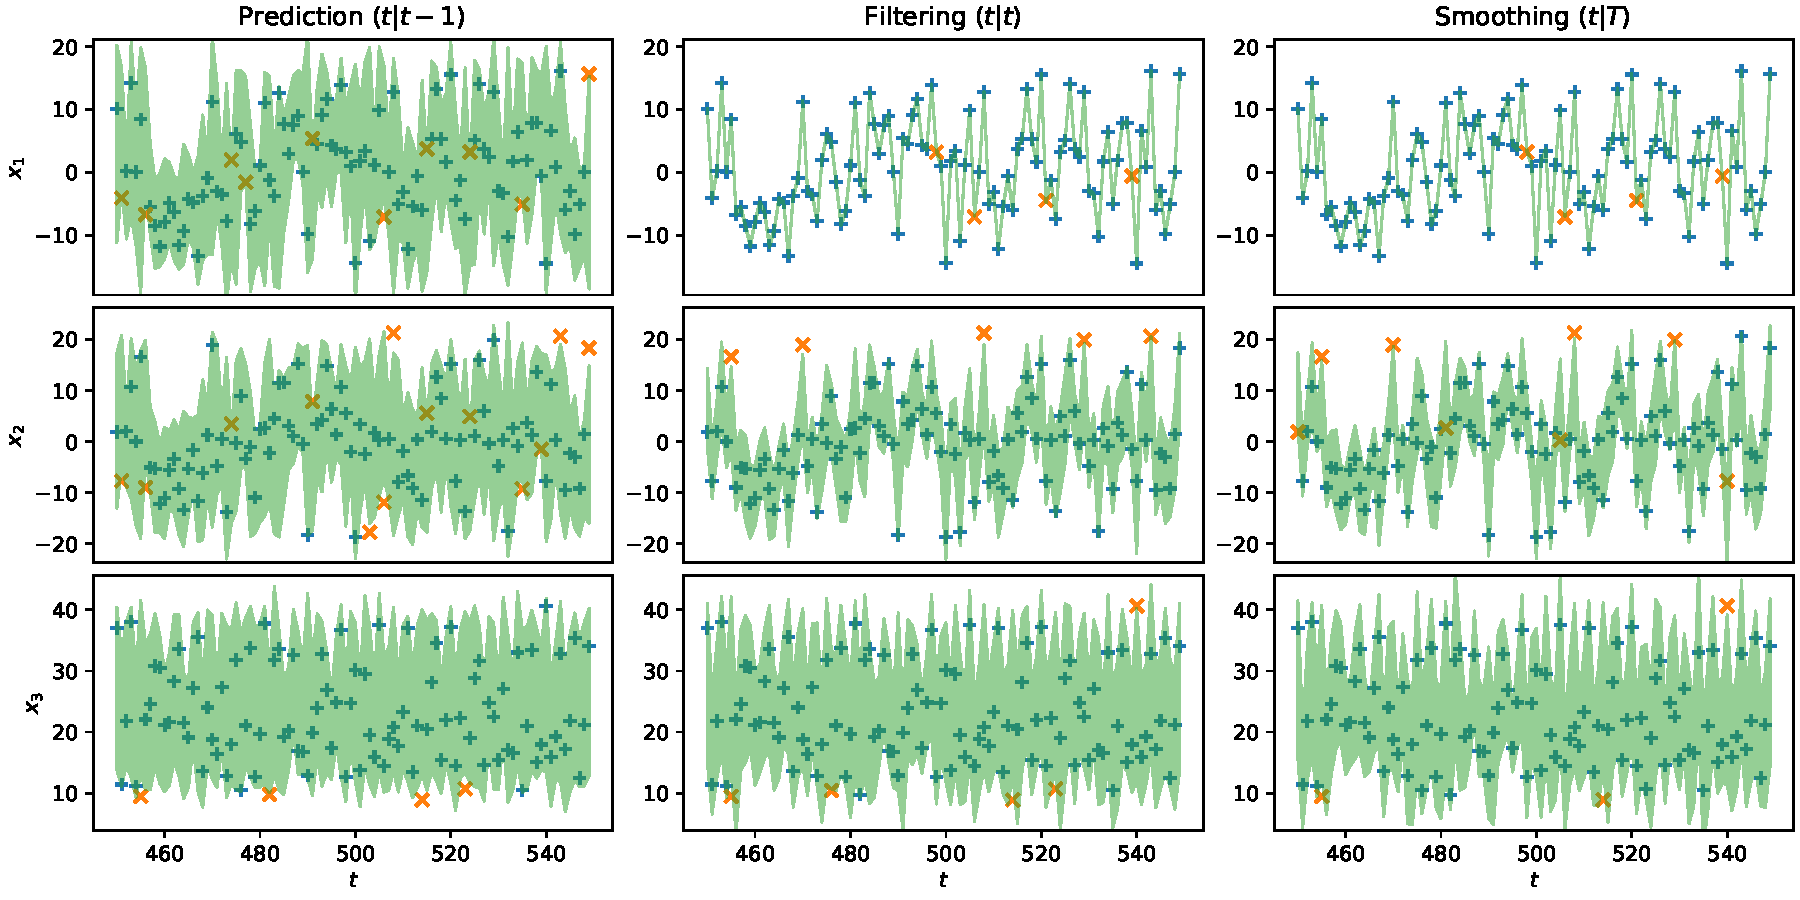
\includegraphics[width=\linewidth]{../figures/analytic-trajectory.pdf}
  \caption{\label{fig:analytic-trajectory} A trajectory excerpt (expect 5 misses) for filtering and smoothing with analytic uncertainty propagation.}
\end{figure}
\begin{figure}
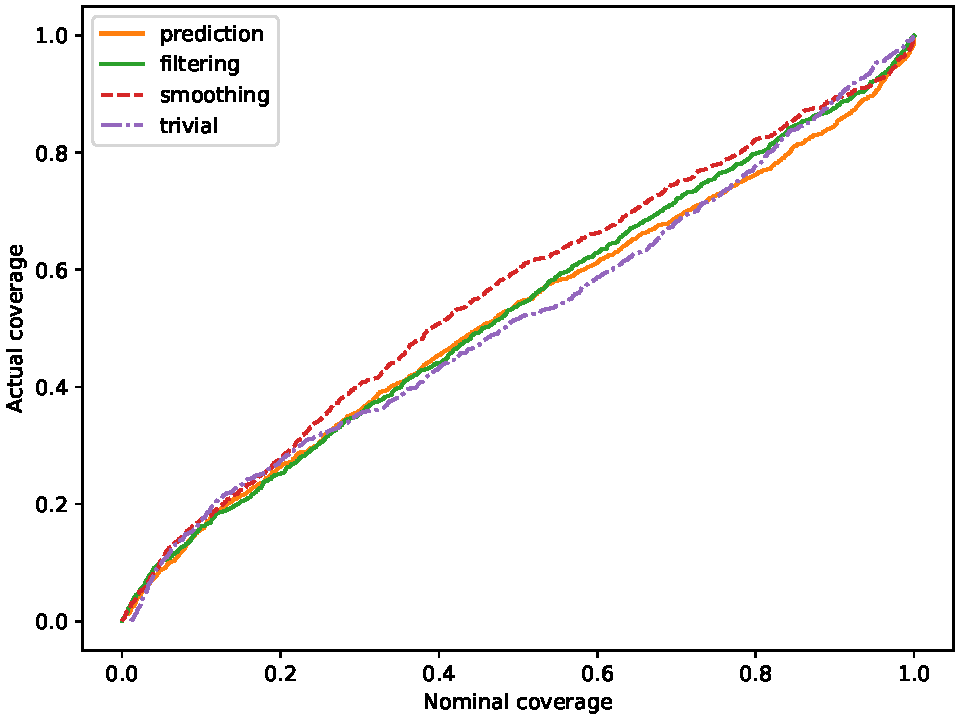
\includegraphics[width=0.5\linewidth]{../figures/analytic-coverage.pdf}
\caption{\label{fig:analytic-coverage} A coverage plot for filtering and smoothing with analytic uncertainty propagation.}
\end{figure}

\appendix
\chapter{Computational complexity}
Rather than reporting runtime, which is highly sensitive to hardware
and implementation, we use JAX ahead-of-time compilation to describe
computational complexity along two axes: input-output operations and
floating point operations.
Comparisons for filtering are shown in
Table~\ref{tab:complexity-predict} and \ref{tab:complexity-update}.
Comparisons for smoothing are shown in Table~\ref{tab:complexity-smooth}.

\begin{table}
  \centering
  \begin{tabular}{lrr}
    \toprule
    Method & I/Os & FLOPs \\
    \midrule
    Analytic & 15\,341\,086 & 25\,269\,848 \\
    Linear & 3\,221\,686 & 14\,943\,866 \\
    Unscented & 469\,652 & 784\,107 \\
    \bottomrule
  \end{tabular}
  \caption{Computational complexity of Filtering \textsc{Predict}}
  \label{tab:complexity-predict}
\end{table}

\begin{table}
  \centering
  \begin{tabular}{lrrr}
    \toprule
    Method & Recalibrate \cite{jiang_new_2025} & I/Os & FLOPs \\
    \midrule
    Analytic & True & 10\,896 & 3\,608 \\
    Linear & True & 4\,488 & 1\,288 \\
    Unscented & True & 9\,595 & 4\,839 \\
    All & False & 393 & 24 \\
    \bottomrule
  \end{tabular}
  \caption{Computational complexity of Filtering \textsc{Update}}
  \label{tab:complexity-update}
\end{table}

\begin{table}
  \centering
  \begin{tabular}{lrr}
    \toprule
    Method & I/Os & FLOPs \\
    \midrule
    Analytic & 16\,309\,000 & 27\,591\,520 \\
    Linear & 3\,447\,040 & 16\,380\,598 \\
    Unscented & 499\,283 & 833\,194 \\
    \bottomrule
  \end{tabular}
  \caption{Computational complexity of Smoothing \textsc{Predict}
  followed by \textsc{Update}}
  \label{tab:complexity-smooth}
\end{table}

\chapter{Derivation of uncertainty propagation formulas for probit activation}
In this appendix, we derive the \(M_\sigma\), \(K_\sigma\), and
\(L_\sigma\) functions (Def~.\ref{def:moment-maps}) for the normal
CDF activation function
\begin{align}
  \sigma(x) &= \sqrt{\frac{2}{\pi}} \int_{0}^x e^{-\frac{1}{2} u^2}
  du = 2 \Phi(x) - 1, \quad \Phi(x) = \probability_{Z \sim \mathcal
  N(0, 1)}(Z \leq x)
  \label{eq:activation}
\end{align}

\begin{definition}
  The bivariate normal CDF \(\Phi_2\) is defined by
  \begin{align*}
    \Phi_2(h, k; \rho)
    &= \probability\sbr{Z_1 \leq h, Z_2\leq k},
    \intertext{where}
    \begin{pmatrix}
      Z_1 \\ Z_2
    \end{pmatrix}
    &\sim \mathcal N\del{\begin{pmatrix} 0 \\ 0 \end{pmatrix}, \begin{pmatrix}
      1 & \rho \\ \rho & 1
    \end{pmatrix}}.
  \end{align*}
\end{definition}
\begin{lemma}
  Let \(M_\sigma\) be defined as in Def.~\ref{def:moment-maps}, with
  \(\sigma\) as in \eqref{eq:activation}.
  \begin{align*}
    M_\sigma(\mu; \nu) &= \sigma\del{\frac{\mu}{\sqrt{1 + \nu}}}
  \end{align*}
  \label{lem:mean}
\end{lemma}
\begin{proof}
  Let \(X \sim \mathcal N(\mu, \nu)\).
  \begin{align}
    \expect \sigma(X)
    &= -1+2\expect \Phi\del{X}
    \\
    &= -1+2\expect \probability \sbr{{Z \leq X} \mid X}
    \tag{introducing an independent \(Z \sim \mathcal{N}(0, 1)\)}
    \\
    &= -1+2\probability\sbr{{Z \leq X}}
    \tag{by the law of total probability}
    \\
    &= -1+2\probability \sbr{Z - X \leq 0}
  \end{align}
  We conclude by noting that the random variable \(Z - X\) has a
  Normal distribution with mean \(-\mu\) and variance \(1 + \nu^2\).
\end{proof}

\begin{lemma}
  Let \(K_\sigma\) be defined as in Def.~\ref{def:moment-maps}, with
  \(\sigma\) as in \eqref{eq:activation}.
  \begin{align*}
    K(\mu_1, \mu_2; \nu_{11}, \nu_{22}, \nu_{12}) &=
    4 \left.
    % \sbr{
    \Phi_2\del{
      \frac{\mu_1}{\sqrt{1 + \nu_{11}}},
      \frac{\mu_2}{\sqrt{1 + \nu_{22}}};
      \rho'
    }
    % }
    \right|^{\rho' = \frac{\nu_{12}}{\sqrt{(1 +
    \nu_{11})(1 + \nu_{22})}}}_{\rho' = 0},
  \end{align*}
  where \(\Phi_2\) is the bivariate normal CDF.
\end{lemma}
\begin{proof}
  Let
  \begin{align}
  \begin{pmatrix} X_1 \\ X_2 \end{pmatrix}
   \sim \mathcal N\left(\begin{pmatrix}
    \mu_1
    \\
    \mu_2
  \end{pmatrix},
  \begin{pmatrix}
    \nu_{11}
    &
    \nu_{12}
    \\
    \nu_{12}
    &
    \nu_{22}
  \end{pmatrix}\right).
  \end{align}
  By a similar calculation as in Lemma~\ref{lem:mean}, we introduce independent
  \(Z_1, Z_2 \sim \mathcal N(0, 1)\) and have
  \begin{align}
    \Cov (\sigma(X_1), \sigma(X_2))
    &= 4 \Cov (\Phi(X_1), \Phi(X_2))
    \\
    &= 4\expect \Phi(X_1) \Phi (X_2) - 4\expect \Phi(X_1) \expect \Phi(X_2)
    \\
    &= 4 \probability\sbr{Z_1 \leq X_1, Z_2 \leq X_2} -
    4\probability\sbr{Z_1 \leq X_1} \probability\sbr{Z_2 \leq X_2}
    \\
    &= 4 \probability\sbr{Z_1 - X_1 \leq 0, Z_2 - X_2 \leq 0} -
    4\probability\sbr{Z_1- X_1\leq 0} \probability\sbr{Z_2 - X_2 \leq 0}.
  \end{align}
  We conclude by using the fact that \((Z_1 - X_1, Z_2 - X_2)\) is
  jointly Normal with distribution
  \begin{align}
    \begin{pmatrix}
      Z_1 - X_1
      \\
      Z_2 - X_1
    \end{pmatrix}
    \sim
    \mathcal{N}\del{
      \begin{pmatrix}
        -\mu_1
        \\
        -\mu_2
      \end{pmatrix},
      \begin{pmatrix}
        1 + \nu_{11}
        &
        \nu_{12}
        \\
        \nu_{12}
        &
        1 + \nu_{22}
      \end{pmatrix}
    }.
  \end{align}
\end{proof}
\begin{remark}
  The bivariate normal CDF can be a difficult transcendental function
  to evaluate.
  Many software packages such as SciPy \cite{wagner_kalman_2022}
  implement the multivariate normal CDF by a (quasi-) Monte Carlo
  integration over \(\mathbb{R}^n\), which is too expensive for our purposes.
  Furthermore, the expression \(\Phi(h, k; \rho) - \Phi(h, k; 0)\) is
  vulnerable to cancellation error for extreme values of \(h\),
  \(k\), and \(\rho\).
  To avoid this, we implement \(K\) by 10-point Gaussian quadrature
  of the one-dimensional proper integral \cite{drezner_computation_1990}
  \begin{align*}
    \Phi_2(h, k; \rho) -
    \Phi_2(h, k; 0)
    &= \int_0^\rho \partial_\rho' \Phi_2(h, k; \rho') \dif\rho',
  \end{align*}
  using
  \begin{align*}
    \partial_\rho \Phi_2(h, k; \rho)
    &= \frac{1}{2\pi \sqrt{1 - \rho^2}} e^{-\frac{1}{2(1 - \rho^2)}
    \del{h^2 + k^2 - 2 \rho h k}}.
  \end{align*}
\end{remark}



\begin{lemma}
  Let \(L_\sigma\) be defined as in Def.~\ref{def:moment-maps}, with
  \(\sigma\) as in \eqref{eq:activation}.
  Then
  \begin{align*}
    L_\sigma(\mu_1, \mu_2; \nu_{11}, \nu_{22}, \nu_{12}) &= 2
    \frac{\nu_{12}}{\sqrt{1 + \nu_{11}}}
    \phi\del{\frac{\mu_1}{\sqrt{1 + \nu_{11}}}}.
  \end{align*}
\end{lemma}
\begin{proof}
   Let
  \begin{align}
  \begin{pmatrix} X_1 \\ X_2 \end{pmatrix}
   \sim \mathcal N\left(\begin{pmatrix}
    \mu_1
    \\
    \mu_2
  \end{pmatrix},
  \begin{pmatrix}
    \nu_{11}
    &
    \nu_{12}
    \\
    \nu_{12}
    &
    \nu_{22}
  \end{pmatrix}\right).
  \end{align}
  Using Lemma \ref{lem:stein}, we have
  \begin{align}
    L_\sigma(\mu_1, \mu_2; \nu_{11}, \nu_{22}, \nu_{12})
    &= \nu_{12} \expect \sigma'(X_1)
    \\
    &= 2\nu_{12} \expect \phi(X_1)
  \end{align}
  where \(\phi = \Phi'\).
  We conclude by appealing to the Gaussian integral identity that
  when \(Z \sim \mathcal N(\mu_Z, \nu_Z)\),
  \begin{align}
    \expect \phi(Z) = \frac{1}{\sqrt{1 + \nu_Z}}
    \phi\del{\frac{\mu_Z}{\sqrt{1 + \nu_Z}}}.
  \end{align}
\end{proof}


\chapter{Derivation of uncertainty propagation formulas for sinusoidal activation}
In this appendix, we derive the \(M_\sigma\), \(K_\sigma\) and
\(L_\sigma\) functions (Def.~\ref{def:moment-maps}) for the sinusoidal activation function
\begin{align}
  \label{eq:activation-sin}
  \sigma(x) &= \sin(x).
\end{align}
We begin by recalling the identities that if \(Z \sim \mathcal N(\mu, \nu)\),
\begin{align}
\label{eq:expect-sin}
  \expect \sin(Z) &= e^{-\nu/2} \sin(\mu)
  \\
  \label{eq:expect-cos}
  \expect \cos(Z) &= e^{-\nu/2} \cos(\mu)
\end{align}

From \eqref{eq:expect-sin} immediately follows:
\begin{lemma}
  Let \(M_\sigma\) be defined as in Def.~\ref{def:moment-maps}, with
  \(\sigma\) as in \eqref{eq:activation-sin}.
  Then
  \begin{align*}
    M_\sigma(\mu; \nu) &= e^{-\nu/2}\sin(\mu).
  \end{align*}
\end{lemma}

\begin{lemma}
  Let \(K_\sigma\) be defined as in Def.~\ref{def:moment-maps}, with
  \(\sigma\) as in \eqref{eq:activation-sin}.
  Then
  \begin{align*}
    K_\sigma(\mu_1, \mu_2; \nu_{11}, \nu_{22}, \nu_{12})
    &= \frac{1}{2} \sbr{e^{\nu^* + \nu_{12}} - e^{\nu^*}} \cos(\mu_1 - \mu_2)
    - \frac{1}{2} \sbr{e^{\nu^* - \nu_{12}} - e^{\nu^*}} \cos(\mu_1 + \mu_2),
    \\
    \intertext{where}
    \nu^* &= -\frac{\nu_{11} + \nu_{22}}{2}.
  \end{align*}
\end{lemma}
\begin{proof}
  Let
  \begin{align}
  \begin{pmatrix} X_1 \\ X_2 \end{pmatrix}
   \sim \mathcal N\left(\begin{pmatrix}
    \mu_1
    \\
    \mu_2
  \end{pmatrix},
  \begin{pmatrix}
    \nu_{11}
    &
    \nu_{12}
    \\
    \nu_{12}
    &
    \nu_{22}
  \end{pmatrix}\right).
  \end{align}
  Then by inserting \eqref{eq:activation-sin}, we have
  \begin{align}
    \Cov(\sigma(X_1), \sigma(X_2))
    &= \expect \sin(X_1) \sin(X_2) - \expect \sin(X_1) \expect \sin(X_2).
    \label{eq:cov-sin-sin}
  \end{align}
  % https://en.wikipedia.org/wiki/List_of_trigonometric_identities#Product-to-sum_and_sum-to-product_identities
  Using some trigonometric identities and \eqref{eq:expect-cos}, the first term of \eqref{eq:cov-sin-sin} becomes
  \begin{align}
    \expect \sin(X_1) \sin(X_2)
    &= \frac{1}{2} \expect \cos(\underbrace{X_1 - X_2}_{
      \mathcal N(\mu_1 - \mu_2, \nu_{11} + \nu_{22} - 2\nu_{12})
      })
    - \frac{1}{2} \expect \cos(\underbrace{X_1 + X_2}_{\mathcal N(\mu_1 + \mu_2, \nu_{11} + \nu_{22} + 2\nu_{12})})
    \\
    &= \frac{1}{2} \exp\del{-\frac{\nu_{11} + \nu_{22}}{2} + \nu_{12}} \cos(\mu_1 - \mu_2)
    - \frac{1}{2} \exp\del{ -\frac{\nu_{11} + \nu_{22}}{2} - \nu_{12}} \cos(\mu_1 + \mu_2)
  \end{align}
  The second term of \eqref{eq:cov-sin-sin} becomes
  \begin{align}
    \expect \sin(X_1) \expect \sin(X_2)
    &= \frac{1}{2} \exp\del{-\frac{\nu_{11} + \nu_{22}}{2}} \cos(\mu_1 - \mu_2)
    - \frac{1}{2} \exp\del{ -\frac{\nu_{11} + \nu_{22}}{2}} \cos(\mu_1 + \mu_2)
  \end{align}
  The result follows from collecting like terms.
\end{proof}

\begin{lemma}
  Let \(L_\sigma\) be defined as in Def.~\ref{def:moment-maps}, with
  \(\sigma\) as in \eqref{eq:activation}.
  Then
  \begin{align*}
    L_\sigma(\mu_1, \mu_2; \nu_{11}, \nu_{22}, \nu_{12})
    &=
    \nu_{12} e^{-\nu_{11}/2} \cos(\mu_1). 
  \end{align*}
\end{lemma}
\begin{proof}
   Let
  \begin{align}
  \begin{pmatrix} X_1 \\ X_2 \end{pmatrix}
   \sim \mathcal N\left(\begin{pmatrix}
    \mu_1
    \\
    \mu_2
  \end{pmatrix},
  \begin{pmatrix}
    \nu_{11}
    &
    \nu_{12}
    \\
    \nu_{12}
    &
    \nu_{22}
  \end{pmatrix}\right).
  \end{align}
  Using Lemma \ref{lem:stein}, we have
  \begin{align}
    L_\sigma(\mu_1, \mu_2; \nu_{11}, \nu_{22}, \nu_{12})
    &= \nu_{12} \expect \sigma'(X_1)
    \\
    &= \nu_{12} \expect \cos(X_1)
    \\
    &= \nu_{12} e^{-\nu_{11}/2} \cos(\mu_1)
  \end{align}
  by \eqref{eq:expect-cos}.
\end{proof}

\clearpage
\chapter{Theoretical guarantees}
The objective of this section is to provide a theoretical analysis of uncertainty propagation through a deep neural network using the formula provided in \eqref{eq:neural-network-gaussian}.
We recall the layer-by-layer Normal approximation resulting in \(Y\) alongside the exact neural network formula resulting in \(Y_0\).
\begin{subequations}
  \begin{align}
    Y &\Longleftarrow Y^\ell & Y_0 &\gets Y^\ell_0
    \\
    Y^k &\Longleftarrow g^k(Y^{k-1}), & Y_0^k &\gets g^k(Y_0^{k-1}), & k \in
    \cbr{1 \ldots \ell},
    \label{eq:hidden-layer-comparison}
    \\
    Y^0 &\Longleftarrow X & Y_0^0 &\gets X,
    \intertext{where \(g^k\) is the function}
    g^k(x) &= g(x; A^k, b^k, C^k, d^k).
\end{align}
\end{subequations}
Recall that the notation \(Y \Longleftarrow X\) means \(Y \gets \mathcal{N}(\expect X, \Var X)\).
Here, the notation \(Y_0^k \gets g^k(Y_0^{k-1})\) means the exact pushforward measure with no Gaussian approximation.
The objective is to analyze the extent to which \(Y \approx Y_0\) in distribution.
In order to avoid taking limits, we will use a statistical distance which
 measures the distance between \(Y\) and \(Y_0\) non-asymptotically.

\begin{definition}
Let \(X\) and \(Y\) be random variables taking values  \(\mathbb{R}^n\).
The Wasserstein distance \(d_\text{W} (\mu, \nu)\) is 
\begin{align*}
  d_\mathrm{W}(X, Y) &= \sup_{\left\|\nabla h\right\|_{\infty} \leq 1} \expect (h(X) - h(Y)).
\end{align*}
\end{definition}

The ultimate goal is to show that \(d_\text{W} (Y_0,Y)\) is small.
We will build up this quantity by recursion through the layers of the neural network.
The key idea is that the error induced by Normal approximation gets worse with every subsequent layer of the network.
% Heuristically, if \(X\) is Normal, then \(Y_0^0\) is close to Normal and therefore well-approximated by its first and second moments.
% Then \(Y_0^1\) is a less Normal than \(Y_0^0\), and so on.
% Thus, roughly speaking, the approximation error in distribution should, by a triangle inequality, scale rougly linearly in the depth of the network.

\subsection{Recursive triangle inequality}
Our basic triangle inequality is
\begin{align}
  \Delta^k &:= d_\mathrm{W}(Y_0^k, Y^k) 
  \label{eq:discrepancy}
  \\
  &= d_\mathrm{W}(g^k(Y_0^{k-1}), Y^k)
  \tag{definition of hidden layer \eqref{eq:hidden-layer-comparison}}
  \\
  &\leq d_\mathrm{W}(g^k(Y_0^{k-1}), g^k(Y^{k-1})) + d_\mathrm{W}(g^k(Y^{k-1}), Y^k)
  \tag{triangle inequality}
  \\
  &\leq \left\|\nabla g^k\right\|_\infty d_\mathrm{W}(Y_0^{k-1}, Y^{k-1}) + d_\mathrm{W}(g^k(Y^{k-1}), Y^k)
  \tag{Lipschitz property of \(d_\mathrm{W}\)}
  \\
  &\leq \left\|\nabla g^k\right\|_\infty \Delta^{k-1} + d_\mathrm{W}(g^k(Y^{k-1}), Y^k)
  \label{eq:discrepancy-recursion}
  % \tag{recursion to \eqref{eq:discrepancy}}
\end{align}
In words, at a hidden layer \(k\),
\begin{multline}
  \text{error at layer \(k\)}
  = \del{\text{Lipschitz constant of layer \(k\)}} \del{\text{error at layer \(k-1\)}} 
  \\
  + \del{\text{normal approximation error at layer \(k\)}}  
\end{multline}
If \(X\) is Gaussian, then \(\Delta^0 = 0\).
We need to fill two blanks to make this formula concrete.

\subsection{Lipschitz constant}
First, the Lipschitz constant \(\left\|\nabla g^k\right\|_\infty\), assuming our convention of \(\sigma = 2\Phi - 1\) as in \eqref{eq:activation}:
\begin{align}
  \nabla g(x; A, b, C, d)
  &= \nabla \sbr{\sigma(A x + b) + C x +  d}
  \\
  % &\leq \left\|A\right\| + \left\|C\right\|.
  &= 2A^\intercal \operatorname{diag} \cbr{\phi(Ax + b)} + C^\intercal
  \intertext{To bound this quantity,}
  \left\|\nabla g(x; A, b, C, d)
  \right\|
  &\leq \sup_{x} \left\|2 A^\intercal \operatorname{diag} \cbr{\phi(Ax + b)} + C^\intercal\right\|
  \\
  &\leq \sqrt{\frac{2}{\pi}} \left\|A\right\|
  + \left\|C\right\|
\end{align}

\subsection{Non-normality}
Second, we need to bound the distance between \(g^k(Y^{k-1})\) and \(Y^k\).
The importance of the recursion \eqref{eq:discrepancy-recursion} is that at layer \(k\), we assess the Normal approximation between \(g^k(Y^{k-1})\), a nonlinear transformation of a Normal random vector, and \(Y^k\), its approximant.
The input to the nonlinearity is Normal.
Since \(Y^{k-1}\) is Normal, we can use techniques from the functional analysis of Gaussian spaces, such as this second-order Poincar\'e inequality:
\begin{theorem}[Second-order Poincar\'e inequality {\cite[Theorem~7.1]{nourdin_second_2009}}]
Suppose that \(Y = f(X)\) is a random vector taking values in \(\mathbb{R}^n\), where \(X\) is a standard Normal random vector, and that \(Y\) has mean \(\mu\) and covariance matrix \(\Sigma\).
Then
\begin{align*}
  d_\mathrm{W}\del{Y, \mathcal N(\mu, \Sigma)}
  \leq \frac{3}{\sqrt 2} \|\Sigma^{-1}\| \|\Sigma\|^{1/2}
  \sbr{\sum_{i = 1}^n \del{\expect \left\|D^2 f_i\right\|^4}^{1/4}}
  \sbr{\sum_{i = 1}^n \del{\expect \left\|D f_i\right\|^4}^{1/4}}
\end{align*}
\end{theorem}

These expectations can be computed exactly with Gaussian integrals.
(WIP)

\bibliographystyle{abbrv}
\bibliography{nn-filtering}
\end{document}